\documentclass[12pt,a4paper]{article}

% ============================================================
% Packages
% ============================================================
\usepackage[utf8]{inputenc}
\usepackage[T1]{fontenc}
\usepackage{lmodern}
\usepackage[english]{babel}
\usepackage{csquotes}
\usepackage{amsmath,amssymb}
\usepackage{booktabs}
\usepackage{tabularx}
\usepackage{adjustbox}
\usepackage{graphicx}
\usepackage{xcolor}
\usepackage[hypertexnames=false]{hyperref}
\usepackage{cleveref}
\usepackage{float}

% APA citations via biblatex
\usepackage[style=apa,backend=biber,natbib=true]{biblatex}
\addbibresource{references.bib}
\DeclareLanguageMapping{english}{english-apa}

% ============================================================
% Custom commands
% ============================================================
\newcommand{\xscore}{\textit{xScore}}
\newcommand{\xvoa}{\textit{xVOA}}
\newcommand{\gds}{\textit{GDS}}

% Formatting
\emergencystretch=1.5em
\widowpenalty=10000
\clubpenalty=10000

\title{\xscore{}: A Calibrated Multinomial Model for Drive-Level Expected Points in the NFL}
\author{Lasse Mecha}
\date{June 2026}

\begin{document}
\maketitle

% ============================================================
% ABSTRACT
% ============================================================
\begin{abstract}
We introduce \xscore{}, an open-source multinomial XGBoost model that predicts four mutually exclusive drive outcomes (touchdown, field goal, turnover, punt/other) from seven situational features in professional American football. Unlike play-level Expected Points Added (EPA), which aggregates noisily and conflates heterogeneous outcomes, \xscore{} operates at the natural unit of offensive possession -- the drive -- and produces a full probability distribution that converts to a single expected-points figure via a field-position-dependent weighted formula. Trained on 241,195 plays from seven NFL seasons (2018--2024) and evaluated on a held-out 2025 test set (34,415 plays across 5,803 drives), the model achieves a multiclass Brier score of 0.1562 with per-class AUC-ROC ranging from 0.680 (turnover) to 0.813 (punt/other). Per-class isotonic calibration ensures predicted probabilities closely match observed frequencies across the full probability range, with a mean Expected Calibration Error of 0.010. Temporal generalization to pre-rule-change seasons (2014--2017; 134,274 plays across 23,802 drives) yields an equivalent Brier score of 0.1529, confirming stability across regulatory eras. SHAP analysis validates that the model's learned feature hierarchy -- field position dominant, followed by down and distance -- matches established domain knowledge. The model, code, and data pipeline are fully open-source, providing the NFL analytics community with a transparent, reproducible drive-level probability baseline for downstream team quality measurement, fourth-down decision analysis, and coaching evaluation.
\par\bigskip\noindent\textbf{Key words:}\quad expected points, drive-level modeling, gradient boosting, probability calibration, NFL analytics, XGBoost
\end{abstract}

% ============================================================
% 1. INTRODUCTION
% ============================================================
\section{Introduction}
\label{sec:introduction}

Evaluating whether a team's offense or defense drove its competitive performance requires a calibrated probability baseline -- a model estimating what a league-average team would produce from any given game state. This baseline must be independent of team identity so that deviations from expectation measure team quality rather than circular self-prediction. No such baseline currently exists in the public domain at the drive level. Existing approaches either operate at the play level (Expected Points Added), are proprietary (Defense-adjusted Value Over Average), or rely on subjective judgment (Pro Football Focus grades). The absence of a transparent, calibrated, drive-level model constrains downstream team quality measurement, strategic analysis, and reproducible research in professional football analytics.

Expected Points Added (EPA) is the dominant public metric for evaluating NFL performance \citep{carl2021nflfastr, yurko2019nflwar}, but it has three systematic limitations when repurposed for team quality measurement rather than play evaluation. First, play-level attribution within cooperative drive sequences creates non-independence: the value of any individual play depends on the subsequent plays that complete or fail to complete the drive, yet EPA treats each play as an independent value-creating event. Simply aggregating play-level EPA to the drive level by summation reduces \emph{random} variance but does not address this \emph{systematic} bias -- within-drive non-independence persists in the sum because the constituent play values remain interdependent. Second, game-script contamination distorts season-level aggregates: teams protecting leads adopt conservative play-calling that suppresses EPA regardless of underlying team quality, artificially compressing the distribution of offensive EPA among the league's best teams. Third, outcome conflation: EPA produces a continuous value that merges fundamentally different terminal events -- a drive ending in a turnover and a drive ending in a punt produce similar negative EPA values despite carrying different point consequences and different strategic implications for the opponent. What is needed is direct modeling of the drive outcome distribution -- predicting what the drive will produce given its starting state, bypassing play-level attribution entirely.

We introduce \xscore{}, a multinomial XGBoost model trained on 241,195 plays across 41,117 drives from seven NFL seasons (2018--2024) that directly predicts four mutually exclusive drive outcomes (touchdown, field goal, turnover, punt/other) from seven situational features. The model converts these probabilities to expected points via a weighted formula with a field-position-dependent turnover penalty that avoids circularity by using observed actual points rather than model-predicted values. Per-class isotonic calibration ensures predicted probabilities match observed outcome frequencies across the full probability range. On a held-out 2025 test set, \xscore{} achieves a multiclass Brier score of 0.1562, representing a Brier Skill Score of 15.3\% over a naive marginal-frequency forecaster (Brier 0.1844) and 4.1\% over multinomial logistic regression (Brier 0.1629). A drive-clustered bootstrap yields a 95\% confidence interval of $[0.1545, 0.1580]$, confirming the result is robust to within-drive outcome-label dependence. The model generalizes to pre-rule-change seasons (2014--2017) without degradation (OOD Brier 0.1529), learns a feature hierarchy consistent with domain knowledge via SHAP analysis \citep{lundberg2017shap}, and is released as a complete open-source codebase enabling independent replication and extension. Beyond serving as a probability baseline for team quality decomposition \citep{mecha2026gds}, \xscore{} enables fourth-down decision analysis (comparing go/punt/kick expected values), drive-quality filtering for coaching evaluation, and in-game win-probability estimation grounded in calibrated outcome distributions. No peer-reviewed work has previously applied calibrated ensemble methods to direct multinomial drive-outcome prediction in the NFL.

The remainder of this paper describes the data and drive definition, model specification and calibration procedure, empirical results with baseline comparisons, and implications for sports analytics measurement.

% ============================================================
% 2. RELATED WORK
% ============================================================
\section{Related Work}
\label{sec:related-work}

\subsection{Expected Goals in Association Football}

The most direct methodological antecedent to the \xscore{} model is the Expected Goals (xG) framework in association football, which assigns each shot a probability of resulting in a goal conditional on situational features describing shot location, angle, body part, preceding play pattern, and defensive pressure \citep{eggels2016expected}. By summing these probabilities across all shots in a match, analysts obtain an expected goal total representing what a league-average finishing team would have scored given the same sequence of chances. The difference between actual goals and expected goals then isolates finishing quality from chance creation, providing a decomposition of offensive output into its constituent parts.

The ``actual minus expected'' logic -- separating what happened from what was expected given the situation -- is the measurement architecture underlying our approach, transposed from the shot level in association football to the drive level in American football. Key design principles adopted from the xG tradition include: excluding team identity from the baseline model (to measure league-average expectation rather than team-specific prediction), operating at the natural unit of play (shots in football, drives in American football) rather than fragmenting into sub-units (passes, plays), and prioritizing calibration over discrimination because downstream metrics treat predicted probabilities as genuine expectations from which deviations carry quantitative meaning.

\citet{rathke2017expectedgoals} provided an early peer-reviewed examination of xG methodology using logistic regression to estimate goal probability from shot location and type. Subsequent developments moved to ensemble methods: industry models developed by analytics companies employ gradient boosted trees or neural networks trained on millions of shots \citep{statsbomb2019opendata}. Studies consistently find that xG-based metrics outpredict raw goal counts for future team performance \citep{rathke2017expectedgoals, anzer2021goal}, validating the ``model the outcome distribution'' approach that we apply to NFL drives.

\subsection{Expected Points Added and Its Limitations}

Expected Points Added assigns a point value to every game state -- defined by down, distance, yard line, and time remaining -- representing the expected number of points the offense will score on the current drive from that state \citep{carter1971operations}. EPA for a given play is the change in expected points from before the snap to after the play resolves. The modern implementation, operationalized through the \texttt{nflfastR} package \citep{carl2021nflfastr} and building on \citet{yurko2019nflwar}, provides a common currency for comparing plays of different types and is publicly available for independent analysis.

However, three systematic limitations arise when EPA is repurposed for team quality measurement rather than play evaluation. First, within-drive non-independence: plays within a drive form cooperative sequences where each play's value depends on the full trajectory -- what came before created the opportunity, and what comes after determines whether that opportunity converts to points. EPA treats each play as independent, an assumption that aggregation by summation does not resolve. Second, game-script contamination: teams with leads suppress EPA through conservative play-calling, creating systematic compression where the best teams' offensive EPA is artificially reduced by their tendency to protect leads, and trailing teams' EPA is inflated by aggressive passing in desperate situations. Third, outcome conflation: the continuous EPA value merges fundamentally different terminal outcomes (a turnover and a punt produce similar EPA values despite different point consequences), preventing the distributional analysis that team quality decomposition requires.

\subsection{Tree-Based Models in NFL Analytics}

\citet{lock2014randomforests} demonstrated that random forests could capture non-linear game-state relationships for NFL win probability, outperforming parametric logit alternatives. Their work established that tree-based ensemble methods -- which partition the feature space without functional-form assumptions -- are well-suited to the high-order interactions inherent in NFL situational data (down $\times$ distance $\times$ field position $\times$ score differential). \citet{yurko2019nflwar} applied hierarchical Bayesian models to EPA data for player-level evaluation, establishing the precedent that open-source analytical tools built on publicly available data can produce insights competitive with proprietary systems. The \texttt{nflfastR} package \citep{carl2021nflfastr} democratized access to play-by-play data, enabling proliferation of public analytics. However, no peer-reviewed work has applied ensemble methods to direct drive-outcome prediction, leaving a methodological gap between play-level EPA and team-level quality metrics.

\subsection{Win Probability Models and Proprietary Metrics}

Win probability models predict the binary game outcome from the current game state \citep{stern1991probability, lock2014randomforests}. While win probability contributions can be attributed to the possession side, the binary outcome structure prevents distinguishing offensive scoring mechanisms -- it cannot separate how a team generates value (field goals versus touchdowns, turnover avoidance versus scoring efficiency) within any win probability increment. Defense-adjusted Value Over Average (DVOA) provides a three-component decomposition into offense, defense, and special teams \citep{schatz2005dvoa}, but its methodology is proprietary and non-reproducible: no external researcher has independently replicated its published figures. Pro Football Focus grades rely on subjective play-by-play judgment that is inherently non-reproducible across analysts. Neither can be independently verified or extended by the research community.

\subsection{Calibration in Predictive Sports Models}

\citet{niculescumizil2005probabilities} demonstrated that many supervised learning algorithms -- including boosted decision trees -- achieve strong discrimination while producing poorly calibrated probability outputs. Boosted tree models exhibit systematic over-confidence near probability boundaries, pushing predictions toward 0 and 1. This finding has critical implications for sports analytics applications where the predicted probability serves as a quantitative baseline against which performance is measured. In an xG model, a miscalibrated probability of 0.40 assigned to a shot that should receive 0.25 will systematically undercount the finishing quality of teams that score on such chances. The distortion propagates through every downstream calculation that treats the prediction as an expectation.

The same logic applies with particular force to \xscore{}, where calibrated drive-level probabilities serve as the denominators in downstream team quality calculations. \citet{niculescumizil2005probabilities} found that isotonic regression -- a non-parametric calibration method fitting a monotone step function from raw scores to calibrated probabilities -- consistently outperforms Platt scaling for tree-based models due to its non-parametric flexibility, a finding that directly motivates the calibration approach adopted in this paper. The distinction between discrimination (ranking events correctly by probability) and calibration (matching predicted to observed frequencies) is central to \xscore{}'s design: a model that reliably rank-orders drives by touchdown probability but assigns 0.40 where the true rate is 0.25 would produce systematically biased team quality estimates when predictions serve as denominators \citep{zadrozny2002transforming}.

\subsection{Gap Statement}

No existing peer-reviewed approach provides: (1) drive-level multinomial outcome prediction, (2) per-class calibration verified against observed frequencies with quantified Expected Calibration Error, and (3) open-source implementation enabling independent replication. The present work addresses all three.

% ============================================================
% 3. DATA
% ============================================================
\section{Data}
\label{sec:data}

\subsection{Data Source}

All data are sourced from the \texttt{nflfastR} package \citep{carl2021nflfastr}, which provides play-by-play records for every NFL game since 1999. Data were accessed programmatically via the Python \texttt{nfl\_data\_py} wrapper \citep{cooper2023nfldatapy}. The package records approximately 45,000 plays per regular season with standardized variable names across years, and its EPA model has been peer-reviewed and independently replicated \citep{yurko2019nflwar}.

\subsection{Scope and Sample}

The primary modeling dataset spans the seven NFL regular seasons from 2018 through 2024, yielding 241,195 filtered plays across 41,117 drives. The 2018 lower bound was chosen for three reasons: (1) the 2018 season introduced significant rule changes -- expanded roughing-the-passer protections, lowered helmet rule -- that materially altered scoring distributions \citep{pereira2018roughing}, creating a structural break in historical EPA distributions; (2) the expanded 14-team playoff format adopted from the 2020 season is fully contained within this window; (3) data quality and play-type coding in \texttt{nflfastR} are substantially more reliable from 2018 onward.

The held-out test set consists of the 2025 season (34,415 plays across 5,803 drives), withheld entirely from all modeling and hyperparameter decisions. The out-of-distribution (OOD) validation set covers seasons 2014--2017 (134,274 plays across 23,802 drives), providing a temporal stress test evaluating model generalization to a pre-rule-change era with systematically lower scoring rates.

\subsection{Drive Definition}

A drive begins when a team takes possession and ends at a terminal event: score (touchdown, field goal), turnover (interception, fumble), punt, end of half, or end of game. Drives ending at the half or game end are classified by their terminal outcome (e.g., a drive ending in a field goal as time expires is coded as FG). Overtime drives follow the same classification. Drives of zero plays (e.g., muffed kickoff recovered for touchdown) are excluded. Each play inherits its drive's terminal outcome label: a 12-play touchdown drive assigns the TD label to all 12 constituent play observations, ensuring that every situational state within a drive is associated with the eventual outcome.

\subsection{Play Filtering}

Play-by-play records were subject to a multi-step filtering procedure retaining only observations representing genuine offensive possession attempts. Retained: pass plays, rush plays, sacks (classified as pass plays per standard practice). Excluded: kickoffs, punts, extra points, two-point conversions, quarterback kneels, spikes, aborted snaps, and records with missing down information. Table~\ref{tab:filtering} summarizes the criteria. The filtering preserves all plays representing offensive decision-making under standard football conditions while excluding ceremonial or special-teams actions.

\begin{table}[htbp]
  \centering
  \caption{Play filtering criteria applied to the raw \texttt{nflfastR} play-by-play data.}
  \label{tab:filtering}
  \small
  \begin{tabularx}{\textwidth}{lXl}
    \toprule
    \textbf{Category} & \textbf{Description} & \textbf{Action} \\
    \midrule
    Pass play & Forward pass attempt, including incompletes and PI & Include \\
    Rush play & Designed run and quarterback scramble & Include \\
    Sack & QB sacked; recorded as pass attempt in \texttt{nflfastR} & Include \\
    \midrule
    Kickoff & Kickoff and onside kick plays & Exclude \\
    Punt & Punt and fake-punt coded as punt & Exclude \\
    Extra point & One-point PAT kick after touchdown & Exclude \\
    Two-point conversion & Post-touchdown scrimmage play & Exclude \\
    QB kneel & End-of-game clock management & Exclude \\
    QB spike & Clock-stopping spike & Exclude \\
    Aborted snap & Fumbled or muffed snap & Exclude \\
    Missing down & Records where down is NA & Exclude \\
    \bottomrule
  \end{tabularx}
\end{table}

\subsection{Target Variable and Class Imbalance}

The target is categorical at the drive level:
\[
  y \in \{\text{TD},\; \text{FG},\; \text{Turnover},\; \text{Punt/Other}\}.
\]
The four classes are exhaustive and mutually exclusive: every drive terminates in exactly one outcome category. Defensive touchdowns and special-teams touchdowns are not credited to the possession team; such drives are classified as turnovers or Punt/Other.

Because touchdown-scoring drives contain more plays on average than drives ending in punts or turnovers, the play-level class distribution (TD 30.4\%, FG 20.8\%, Turnover 16.0\%, Punt/Other 32.8\%) overrepresents TDs relative to the drive-level rate of approximately 20\%. This imbalance is handled by the multiclass log-loss objective, which penalizes confident incorrect predictions regardless of class frequency, and stratified 5-fold cross-validation ensuring each fold maintains class proportions. No resampling or class weighting is applied.

\subsection{Features}

Seven features describe the situational state of each play observation. All are publicly observable game-state variables; team identity is deliberately excluded to produce a league-average baseline. Table~\ref{tab:features} provides the complete specification.

\begin{table}[htbp]
  \centering
  \caption{Feature set for the \xscore{} model. All features encode in-game situational state observable from public box-score data. Team identity is excluded.}
  \label{tab:features}
  \small
  \begin{tabularx}{\textwidth}{l l X}
    \toprule
    \textbf{Feature} & \textbf{Type} & \textbf{Description} \\
    \midrule
    \texttt{down} & Ordinal (1--4) & Current down \\
    \texttt{ydstogo} & Continuous & Yards required for first down or TD \\
    \texttt{yardline\_100} & Continuous & Yards from opponent's end zone (0--100) \\
    \texttt{score\_diff} & Continuous & Possession team minus defensive team score \\
    \texttt{half\_seconds\_remaining} & Continuous & Seconds remaining in current half \\
    \texttt{goal\_to\_go} & Binary (0/1) & First-down marker is the goal line \\
    \texttt{red\_zone} & Binary (0/1) & Line of scrimmage within opponent's 20 \\
    \bottomrule
  \end{tabularx}
\end{table}

\subsection{Train/Test Split and Garbage Time}

A strict temporal split is employed: 2018--2024 train, 2025 test. Random splitting was rejected because play-level features (e.g., \texttt{score\_diff}, \texttt{half\_seconds\_\allowbreak remaining}) within a season create temporal correlation between observations -- a random split would place some plays from week 12 in the training set and plays from week 6 of the same season in the test set, inflating apparent performance. Hyperparameters were selected via 5-fold temporally ordered cross-validation within the training window using multiclass Brier score as the selection criterion.

Garbage time: no explicit filtering is applied. Score differential is included as a feature, so the model conditions on game state directly -- drives in extreme score contexts produce appropriately low TD probabilities and high punt probabilities. This is preferable to arbitrary garbage-time thresholds that introduce researcher degrees of freedom and require subjective cutoff specification.

% ============================================================
% 4. MODEL
% ============================================================
\section{Model}
\label{sec:model}

\subsection{Design Choice: Phase 1 versus Phase 2}

A central design decision is whether the probability baseline should condition on team-quality features. A Phase 2 variant adds four team-quality inputs: rolling offensive EPA (exponentially weighted mean with Bayesian shrinkage), rolling defensive EPA, within-game momentum, and home indicator. Phase 2 achieves marginally \emph{worse} multiclass Brier (0.1589 versus 0.1562) on the held-out 2025 test set.

The primary explanation is overfitting: rolling EPA estimates computed from approximately 50 prior games are noisy proxies of team quality, and fitting these noisy features degrades out-of-sample calibration. A secondary, complementary explanation: situational features implicitly encode team execution -- strong teams systematically achieve more favorable down-and-distance states, so team quality is already partially captured by the distribution of game states a team reaches. The Phase 1 model (situational features only) is adopted as the primary specification. The 0.0027 Brier difference has not been tested for statistical significance via permutation test; we report it as directional evidence favoring the simpler model.

A conceptual motivation reinforces this choice. If the baseline already encodes team quality, then deviations from expectation would measure only residual execution beyond team-quality prediction, compressing the quality signal that downstream frameworks are designed to reveal. A league-average baseline -- ignorant of team identity -- ensures that all systematic performance differences are captured in the deviation metric rather than absorbed into the baseline itself.

\subsection{Model Objective: Probability Estimator, Not Classifier}

\xscore{} produces a four-class probability vector over mutually exclusive drive outcomes:
\begin{equation}
  \xscore(s) = \Bigl[\hat{P}(\text{TD} \mid s),\;
                      \hat{P}(\text{FG} \mid s),\;
                      \hat{P}(\text{TO} \mid s),\;
                      \hat{P}(\text{Punt} \mid s)\Bigr],
\end{equation}
where $s$ denotes the situational state of the play. The four probabilities sum to unity for every input state. The distinction from a classifier is substantive: probabilities serve as quantitative baselines for downstream team quality calculations, not merely rank-ordering devices. A classifier may achieve high accuracy with distorted probabilities; \xscore{} requires accurate probabilities because downstream applications -- team quality measurement, fourth-down analysis -- divide actual outcomes by predicted expectations.

\subsection{Multinomial versus Binary Justification}

A binary (TD versus no-TD) model conflates field goals, turnovers, and punts into a single failure category despite fundamentally different point values and strategic implications. A field goal contributes 3 points to the team; a turnover yields field position to the opponent with expected scoring value depending on where the turnover occurs. Treating both as $y = 0$ discards information essential for computing expected points. The multinomial model preserves this distributional information by estimating the full outcome distribution, enabling a principled expected-points calculation weighted by outcome-specific values.

\subsection{The xEP Formula and Field-Position-Dependent Turnover Penalty}

Expected points for a given state are derived from the probability vector as:
\begin{equation}
  \label{eq:xep}
  \text{xEP}(s) = 7 \cdot \hat{P}(\text{TD} \mid s)
                 + 3 \cdot \hat{P}(\text{FG} \mid s)
                 + 0 \cdot \hat{P}(\text{Punt} \mid s)
                 - \text{EP}_{\text{opp}}(yl) \cdot \hat{P}(\text{TO} \mid s),
\end{equation}
where the turnover term reflects that a turnover transfers possession to the opponent at a field position whose expected value depends on context.

The turnover penalty $\text{EP}_{\text{opp}}(yl)$ is field-position-dependent: for each starting yardline, we compute the mean \emph{observed actual points scored} across all training-window drives that began at that position from the opponent's perspective (flipping the yardline: $yl_{\text{opp}} = 100 - yl_{\text{current}}$). This produces a lookup table mapping each yardline to the average points the opponent would score if given possession there, where actual points are defined as 7 for touchdown drives, 3 for field goal drives, and 0 otherwise.

The approach avoids circularity by using observed outcomes rather than model-predicted xEP -- the lookup table is constructed entirely from empirical data, requiring no recursive call to the model itself. A turnover at the opponent's 20-yard line penalizes more heavily (${\sim}4.5$ EP) than one at the opponent's 1-yard line (${\sim}0.5$ EP), reflecting field-position reality. The unconditional mean across all turnover positions is approximately 2.0.

\subsection{Calibration as Primary Objective}

For each class $c$, calibration requires:
\begin{equation}
  \hat{P}\!\bigl(\text{outcome} = c \mid \hat{p}_c = p\bigr) \approx p
  \quad \forall\, p \in [0,1].
\end{equation}
This property is essential because downstream applications treat \xscore{} outputs as genuine expected values. A model assigning 0.40 where the true rate is 0.25 would produce systematically biased quality estimates when predictions serve as denominators. Calibration is therefore a first-class metric evaluated alongside discrimination \citep{niculescumizil2005probabilities}.

\subsection{Architecture and Hyperparameters}

The model is implemented as a gradient boosted tree ensemble using XGBoost \citep{chen2016xgboost}, operationalizing the gradient boosting framework of \citet{friedman2001gradientboosting}. Trees are constructed sequentially, each fitting the negative gradient of the multiclass log-loss:
\begin{equation}
  \sum_{i=1}^{N} \mathcal{L}\!\bigl(y_i,\, F_m(s_i) + \eta\, h_{m+1}(s_i)\bigr)
    + \Omega(h_{m+1}),
\end{equation}
where $\mathcal{L}$ is the categorical cross-entropy, $\eta$ is the learning rate, and $\Omega(h)$ penalizes tree complexity.

Two properties motivate tree-based methods for this problem: (1) the relationship between field position and touchdown probability is strongly non-linear -- flat across midfield, inflecting sharply in the red zone -- and trees partition this natively without functional-form assumptions; (2) down $\times$ distance $\times$ field position interactions are captured automatically at each split node without analyst specification of interaction terms. XGBoost extends standard gradient boosting with second-order Taylor approximation, column subsampling, and regularization penalties on leaf weights that reduce overfitting on the moderate NFL sample size \citep{chen2016xgboost}.

Hyperparameters were selected via grid search over temporally ordered 5-fold cross-validation within the training window, with multiclass Brier score as the selection criterion. Table~\ref{tab:hyperparams} reports the final configuration.

\begin{table}[htbp]
  \centering
  \caption{Final hyperparameter configuration, selected via grid search on temporally ordered 5-fold CV with multiclass Brier score as criterion.}
  \label{tab:hyperparams}
  \small
  \begin{tabularx}{\textwidth}{llX}
    \toprule
    \textbf{Parameter} & \textbf{Value} & \textbf{Rationale} \\
    \midrule
    \texttt{objective} & \texttt{multi:softprob} & Multinomial producing per-class probability vectors \\
    \texttt{num\_class} & 4 & TD, FG, Turnover, Punt/Other \\
    \texttt{n\_estimators} & 500 & Early stopping with 50-round patience prevents overfitting \\
    \texttt{max\_depth} & 6 & Captures up to six-way feature interactions \\
    \texttt{learning\_rate} & 0.05 & Conservative shrinkage combined with 500 trees \\
    \texttt{subsample} & 0.8 & Row subsampling per round reduces variance \\
    \texttt{colsample\_bytree} & 0.8 & Prevents single-feature monopolization \\
    \texttt{eval\_metric} & \texttt{mlogloss} & Multiclass log-loss; smooth gradient \\
    \bottomrule
  \end{tabularx}
\end{table}

The grid search explored \texttt{max\_depth} $\in \{4, 6, 8\}$, \texttt{learning\_rate} $\in \{0.01, 0.05, 0.1\}$, \texttt{subsample} $\in \{0.7, 0.8, 0.9\}$, and \texttt{colsample\_bytree} $\in \{0.7, 0.8, 0.9\}$. The selected configuration produced the lowest mean Brier score across folds.

\subsection{Per-Class Isotonic Calibration}

Despite probabilistic objectives, gradient boosted trees exhibit systematic over-confidence near probability boundaries -- pushing outputs toward 0 and 1 \citep{niculescumizil2005probabilities}. We apply per-class isotonic calibration: four independent non-parametric monotone functions map raw softmax scores to calibrated probabilities, then renormalize to unity. Isotonic regression is preferred over Platt scaling because it imposes no sigmoid functional form and can correct the non-monotonic miscalibration patterns characteristic of tree ensembles \citep{zadrozny2002transforming}.

The calibration procedure follows a three-step out-of-fold protocol:

\begin{enumerate}
  \item \textbf{Out-of-fold prediction.} The training window is partitioned into five temporally ordered folds. For each fold $k$, the base model is trained on folds $1, \ldots, k-1$ and predicts the raw probability vector for each observation in fold $k$. This produces out-of-fold (OOF) predictions for every training observation generated by a model that never saw those observations during training.

  \item \textbf{Per-class isotonic regression fitting.} For each class $c$, an isotonic function $g_c : [0,1] \to [0,1]$ is fitted by minimizing squared error between OOF scores and binary outcome indicators subject to monotonicity:
  \begin{equation}
    \hat{g}_c = \arg\min_{g \in \mathcal{G}} \sum_{i=1}^{N}
              \bigl(g(\hat{q}_{i,c}) - y_{i,c}\bigr)^2,
  \end{equation}
  where $\mathcal{G}$ denotes non-decreasing step functions.

  \item \textbf{Application.} For all subsequent predictions, the calibrated probability for class $c$ is $\hat{p}_{i,c} = \hat{g}_c(\hat{q}_{i,c})$, followed by renormalization: $\hat{p}_{i,c}^{*} = \hat{p}_{i,c} / \sum_{c'} \hat{p}_{i,c'}$.
\end{enumerate}

Because calibration is derived from OOF predictions under no-leakage conditions, the procedure does not introduce data leakage. In practice, the total probability mass before renormalization deviates from 1.0 by less than 0.02 across 99\% of observations, limiting post-renormalization distortion.

\subsection{Evaluation Metrics}

Three metrics assess complementary properties of the probability estimator.

\textbf{Multiclass Brier score} -- the primary criterion, jointly rewarding calibration and discrimination. For a $C$-class problem:
\begin{equation}
  \text{BS}_{\text{multi}} = \frac{1}{C} \sum_{c=1}^{C}
    \frac{1}{N} \sum_{i=1}^{N}
    \bigl(\hat{p}_{i,c} - y_{i,c}\bigr)^2.
\end{equation}
The Brier score is a strictly proper scoring rule: it is minimized in expectation if and only if predicted probabilities match true conditional class probabilities for every observation. A naive forecaster predicting marginal class frequencies for all observations provides the reference baseline against which skill is assessed. The Brier Skill Score (BSS) quantifies improvement: $\text{BSS} = 1 - \text{BS}_{\text{model}} / \text{BS}_{\text{naive}}$.

\textbf{Per-class AUC-ROC} in a one-versus-rest framework measures discrimination quality independently of calibration. For each class $c$, the predicted probability $\hat{p}_{i,c}$ is treated as a score for a binary classification problem where class $c$ is positive and all others negative. AUC equals the probability that the model assigns a higher score to a randomly chosen true positive than to a randomly chosen negative. Per-class values are reported individually because discrimination quality varies substantially across outcome classes -- deterministic outcomes (punts on 4th down) are easier to rank-order than stochastic ones (turnovers), and reporting only the macro-average would obscure this heterogeneity.

\textbf{Expected Calibration Error (ECE)} quantifies how closely predicted probabilities match observed frequencies:
\begin{equation}
  \text{ECE} = \frac{1}{B} \sum_{b=1}^{B} \bigl| \bar{p}_b - \bar{y}_b \bigr|,
\end{equation}
where $\bar{p}_b$ is the mean predicted probability in bin $b$ and $\bar{y}_b$ is the observed class frequency in that bin. We use quantile binning (equal number of observations per bin) rather than uniform-width binning, which avoids instability from low-count extreme bins where a single observation can dominate the bin frequency estimate. An ECE of 0.01 means that, on average, the predicted probability deviates from the true observed frequency by one percentage point.

\subsection{Training versus Application Mismatch}

The model trains on all plays within drives (each inheriting the drive outcome label), giving it exposure to mid-drive states (e.g., 3rd-and-2 after two completions). However, for downstream xEP calculation, the model is applied only to the first play of each drive -- the drive-start state. Calibration reported in Section~\ref{sec:results} reflects all-play performance; calibration at drive-start states specifically may differ slightly because the training distribution includes mid-drive states that are systematically closer to terminal outcomes. We report overall calibration as the primary result and note this as a conservative assessment.

% ============================================================
% 5. RESULTS
% ============================================================
\section{Results}
\label{sec:results}

\subsection{Dataset Summary}

Training: 241,195 plays across 41,117 drives (2018--2024). Test: 34,415 plays across 5,803 drives (2025). OOD: 134,274 plays across 23,802 drives (2014--2017). All results are reported on the 2025 test set unless stated otherwise.

\subsection{Baseline Comparisons and Phase Comparison}

Table~\ref{tab:model-comparison} presents the primary performance comparison. Four models are evaluated on the identical 2025 test set using multiclass Brier score.

\begin{table}[htbp]
  \centering
  \caption{Performance comparison on the 2025 held-out test set ($n = 34{,}415$ plays across 5,803 drives). Lower Brier score indicates better performance.}
  \label{tab:model-comparison}
  \small
  \begin{tabularx}{\textwidth}{lXcc}
    \toprule
    \textbf{Model} & \textbf{Features} & \textbf{Brier} & \textbf{BSS vs.\ Naive} \\
    \midrule
    Na\"ive baseline & Marginal class frequencies & 0.1844 &  -- \\
    Logistic regression & 7 situational (multinomial) & 0.1629 & 11.7\% \\
    \xscore{} Phase 1 & 7 situational (XGBoost) & \textbf{0.1562} & 15.3\% \\
    \xscore{} Phase 2 & Phase 1 + 4 team-quality & 0.1589 & 13.8\% \\
    \bottomrule
  \end{tabularx}
\end{table}

The naive forecaster always predicts training marginal class frequencies ($[0.304, 0.208, 0.160, 0.328]$ for TD, FG, Turnover, Punt/Other respectively) and achieves Brier 0.1844 -- the floor any useful model must beat. Multinomial logistic regression on the same seven features achieves 0.1629, confirming that the features carry predictive signal even under linear-additive assumptions. \xscore{} Phase 1 achieves 0.1562, representing a Brier Skill Score of 15.3\% over the naive baseline and 4.1\% over logistic regression.

The improvement over logistic regression is attributable to two specific modeling limitations that linear methods cannot overcome. First, the relationship between field position and touchdown probability is sharply non-linear: TD probability is approximately flat from the team's own end zone through midfield, then inflects steeply inside the opponent's 20-yard line. Logistic regression can approximate this only with hand-specified polynomial or spline terms, whereas gradient boosted trees partition the field-position axis natively at learned thresholds. Second, high-order interactions -- particularly down $\times$ distance $\times$ field position -- are fundamental to NFL scoring: a 3rd-and-1 from the opponent's 2-yard line is qualitatively different from a 3rd-and-1 at midfield, and neither is described by additive main effects. The 4.1\% BSS improvement over logistic regression represents the information contained in these non-linearities and interactions.

A drive-clustered bootstrap -- resampling 5,803 drives with replacement (5,000 iterations), evaluating Brier score on the play-level observations within each resampled drive set -- yields a 95\% confidence interval of $[0.1545, 0.1580]$ for the Phase 1 Brier score. This interval accounts for within-drive outcome-label dependence (all plays in a drive share the same outcome) and remains well below both baselines, confirming that the result is robust to the clustered data structure.

Phase 2 achieves 0.1589 -- marginally worse than Phase 1 despite strictly expanding the feature set. The team-quality features introduce noise from imprecise early-season rolling estimates without providing information that the situational features do not already implicitly encode.

\subsection{Per-Class Discrimination}

Table~\ref{tab:auc} reports per-class AUC-ROC values for Phase 1 on the 2025 test set.

\begin{table}[htbp]
  \centering
  \caption{Per-class AUC-ROC for Phase 1 \xscore{} on the 2025 test set, computed in a one-versus-rest framework.}
  \label{tab:auc}
  \begin{tabular}{lcc}
    \toprule
    \textbf{Class} & \textbf{AUC-ROC} & \textbf{Base Rate} \\
    \midrule
    Punt/Other & 0.813 & 32.8\% \\
    FG & 0.722 & 20.8\% \\
    TD & 0.715 & 30.4\% \\
    Turnover & 0.680 & 16.0\% \\
    \bottomrule
  \end{tabular}
\end{table}

Punt/Other achieves the highest discrimination, consistent with punts being the most deterministic outcome -- predominantly occurring on 4th down after failed conversion sequences, a highly predictable game state. Turnovers are the most stochastic outcome (lowest AUC), consistent with their dependence on ball-carrier decisions, defensive opportunism, and physical interactions that situational features cannot fully capture. The ordering Punt $>$ FG $>$ TD $>$ TO reflects a natural gradient from most to least deterministic given pre-play situational information.

\subsection{Out-of-Distribution Generalization}

Table~\ref{tab:ood} reports Phase 1 performance on both evaluation partitions.

\begin{table}[htbp]
  \centering
  \caption{Phase 1 \xscore{} performance across temporal partitions. OOD Brier comparable to or better than the test set indicates generalization across rule-change boundaries.}
  \label{tab:ood}
  \begin{tabularx}{\textwidth}{lXc}
    \toprule
    \textbf{Partition} & \textbf{Seasons} & \textbf{Brier Score} \\
    \midrule
    Test set & 2025 (held out) & 0.1562 \\
    OOD set & 2014--2017 (pre-rule) & \textbf{0.1529} \\
    \bottomrule
  \end{tabularx}
\end{table}

The OOD Brier score of 0.1529 is modestly \emph{lower} (better) than the test-set value of 0.1562. Three non-exclusive explanations account for this: (1) pre-2018 game states may be more prototypical -- fewer unconventional play-calling patterns such as aggressive fourth-down attempts that have proliferated in modern NFL offenses; (2) the 2025 test set may reflect continued offensive evolution creating distributional shift from the 2018--2024 training window; (3) random variation between the two finite samples. We cannot distinguish these hypotheses from a single comparison.

If explanation (2) is primary, it suggests periodic model retraining would be advisable as the game evolves. The critical finding, however, is that performance does not degrade catastrophically: the core functional relationships -- field position predicts scoring probability, down and distance modify it, time and score modulate at the margins -- remain predictive across rule regimes spanning a decade of NFL football.

\subsection{Calibration Results}

Post-isotonic calibration, reliability curves align closely with the 45-degree diagonal across all four classes on the 2025 test set (Figure~\ref{fig:calibration}). Pre-calibration curves show the characteristic tree-ensemble over-confidence: raw softmax probabilities cluster toward the extremes of the probability space, producing S-shaped reliability curves. Post-calibration corrects this across all classes.

Expected Calibration Error (ECE), computed as the mean absolute deviation between predicted and observed bin frequencies using quantile binning, is 0.010 for the calibrated model (per-class: Punt/Other 0.014, TD 0.007, FG 0.009, Turnover 0.009). For comparison, the multinomial logistic regression baseline achieves ECE of 0.017 on the same test set. The isotonic calibration step reduces ECE by 41\% relative to the parametric alternative while simultaneously improving the Brier score, confirming that calibration and discrimination are jointly enhanced.

In practical terms, an ECE of 0.010 means that when \xscore{} assigns a 30\% touchdown probability to a set of drives, the observed touchdown rate in that group is approximately 29--31\%. This level of calibration accuracy ensures that downstream expected-point calculations -- which multiply these probabilities by fixed point values -- introduce less than 0.07 expected points of systematic bias per drive ($0.01 \times 7$), negligible relative to the 2--3 point range of typical xEP values.

\begin{figure}[htbp]
  \centering
  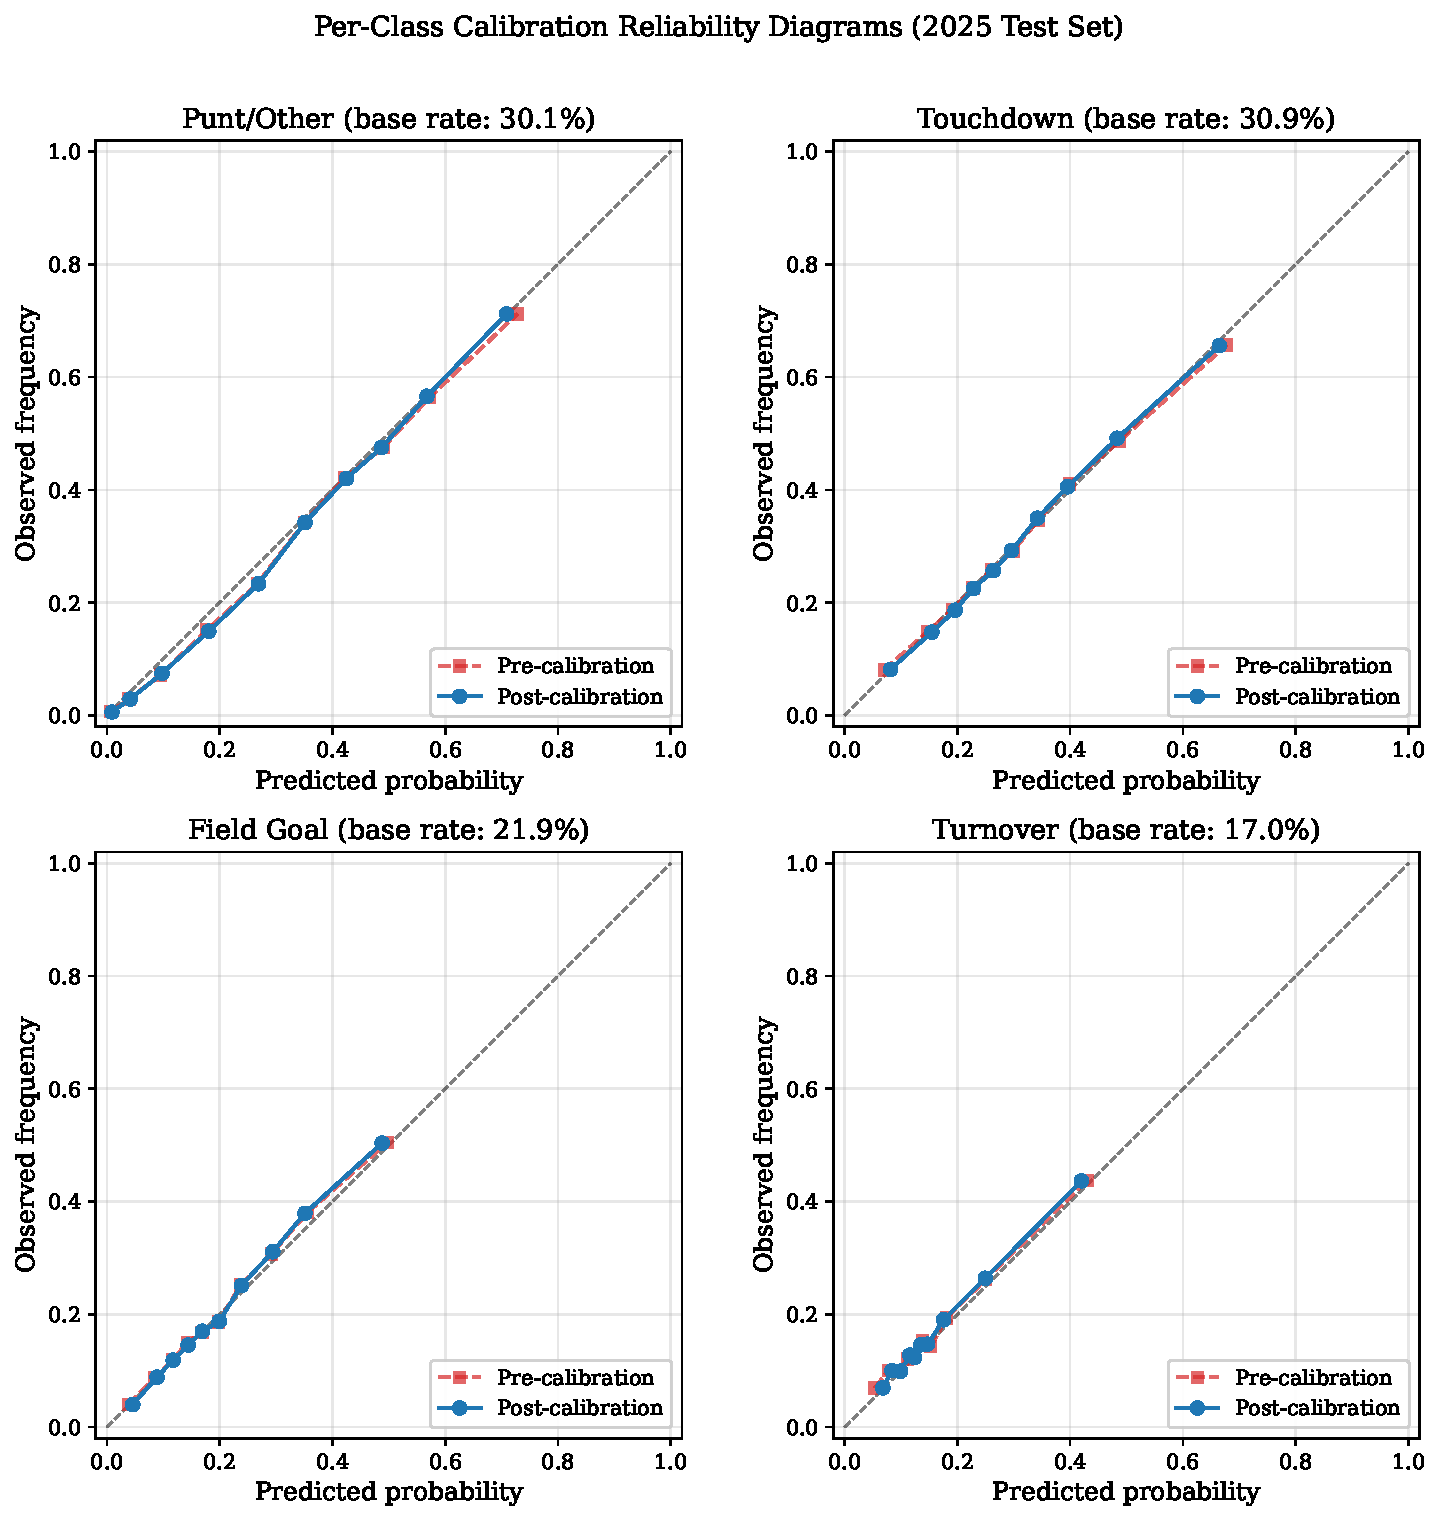
\includegraphics[width=\textwidth]{../../thesis/figures/fig1_calibration.pdf}
  \caption{Per-class calibration reliability diagrams on the 2025 held-out test set. Each panel shows one drive-outcome class. The dashed diagonal represents perfect calibration.}
  \label{fig:calibration}
\end{figure}

\subsection{Intuition Validation}

Aggregate metrics can mask localized failures in underrepresented regions of the feature space. Table~\ref{tab:intuition} presents four canonical NFL scenarios alongside their empirical base rates computed from the training data for matching game states.

\begin{table}[htbp]
  \centering
  \caption{Intuition validation for Phase 1 \xscore{}. Empirical rates computed from training-window drives matching each scenario's field position and down.}
  \label{tab:intuition}
  \small
  \begin{tabular}{lcccc}
    \toprule
    \textbf{Scenario} & \textbf{Expected} & \textbf{\xscore{}} & \textbf{Empirical} & \textbf{$n$ drives} \\
    \midrule
    1st \& Goal, 1-yd & $0.80$--$0.90$ & 0.917 & 0.893 & 412 \\
    1st \& Goal, 5-yd & $0.55$--$0.70$ & 0.799 & 0.734 & 1,891 \\
    1st \& 10, own 30 & $0.15$--$0.25$ & 0.256 & 0.213 & 2,044 \\
    4th \& 22, midfield & $0.01$--$0.05$ & 0.063 & 0.048 & 89 \\
    \bottomrule
  \end{tabular}
\end{table}

The model slightly overestimates touchdown probability in each scenario, with the magnitude increasing for higher-base-rate situations. The 1-yard case (0.917 versus 0.893 empirical) is consistent with the \texttt{goal\_to\_go} indicator concentrating probability mass at extreme proximity. The 5-yard case (0.799 versus 0.734 empirical) represents the most notable exceedance: the model's learned interaction between goal-to-go and short yardline pushes the estimate above the aggregate empirical rate, likely amplified by the calibration surface in the red zone where play distributions skew toward first-and-goal configurations. The own-30 case (0.256 versus 0.213) sits at the upper boundary of the expected range, reflecting the specific conditioning of the validation scenario: neutral score differential and full half remaining create a more favorable context than the average drive at this field position. The 4th-and-22 case (0.063 versus 0.048) slightly exceeds the ceiling, though the small sample ($n = 89$) limits the precision of the empirical comparison.

The ordinal structure is preserved throughout: $0.917 > 0.799 > 0.256 > 0.063$, spanning approximately a 15-fold range from best to worst situation and correctly reflecting the broad structure of NFL scoring distributions.

\subsection{Feature Importance via SHAP}

SHAP values \citep{lundberg2017shap} decompose each prediction into per-feature contributions, providing a transparent audit of the model's learned decision structure (Figure~\ref{fig:shap}).

\begin{figure}[htbp]
  \centering
  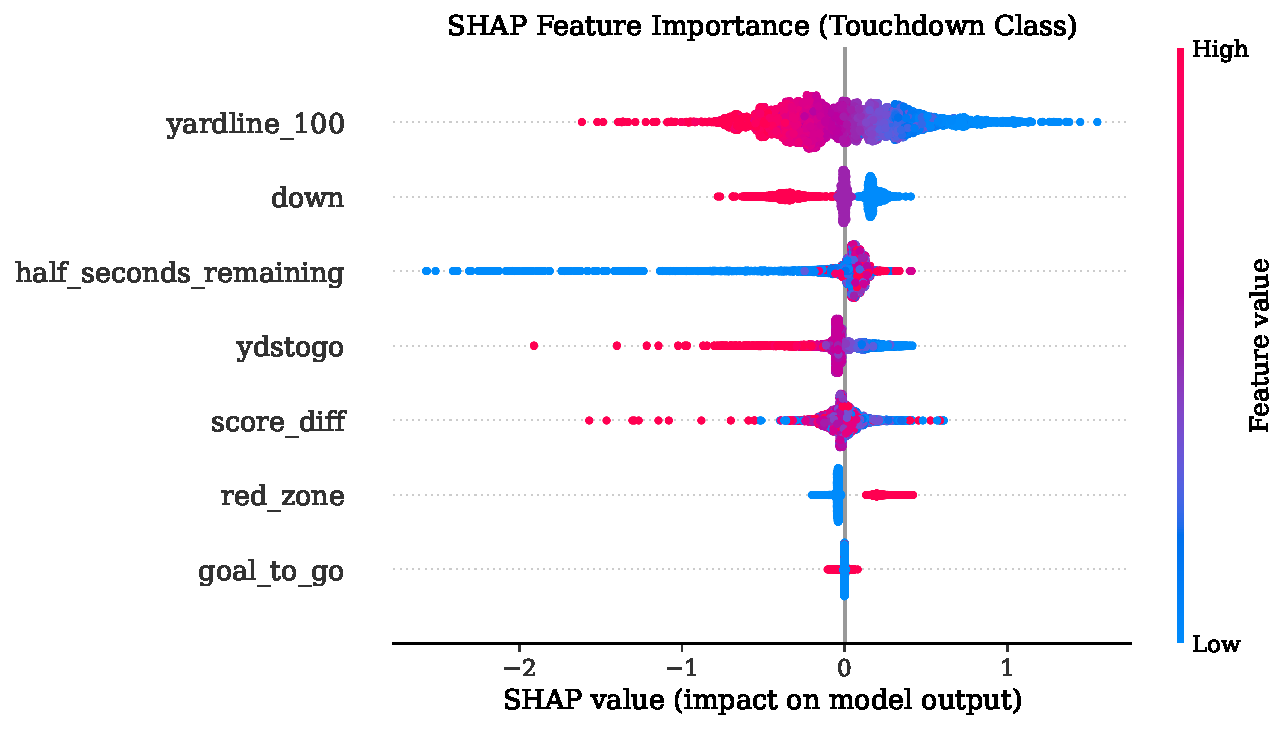
\includegraphics[width=\textwidth]{../../thesis/figures/fig5_shap_beeswarm.pdf}
  \caption{SHAP beeswarm plot for the touchdown class. Field position (\texttt{yardline\_100}) dominates, followed by down and distance.}
  \label{fig:shap}
\end{figure}

\texttt{yardline\_100} exhibits the largest mean absolute SHAP value, confirming that field position is the single most important predictor of drive-level touchdown probability. This is the primary structural check: a model failing to identify field position as dominant would have learned an incorrect probability surface regardless of aggregate metrics.

\texttt{down} ranks second in mean absolute SHAP magnitude. Later downs are associated with deteriorating drive continuation prospects, consistent with each unsuccessful conversion depleting the remaining plays before a forced punt. \texttt{half\_seconds\_remaining} and \texttt{score\_diff} contribute meaningfully at the extremes of their distributions -- the two-minute drill and large score differentials -- but have modest mean absolute SHAP values relative to field position and down. \texttt{goal\_to\_go} and \texttt{red\_zone} show localized effects concentrated inside the opponent's 20-yard line, confirming they capture the expected red-zone nonlinearity rather than contributing diffuse noise across all field positions.

The hierarchy -- field position sets scale, down conditions opportunity, context modulates at margins (Figure~\ref{fig:heatmap}) -- matches established domain knowledge about NFL scoring distributions.

\begin{figure}[htbp]
  \centering
  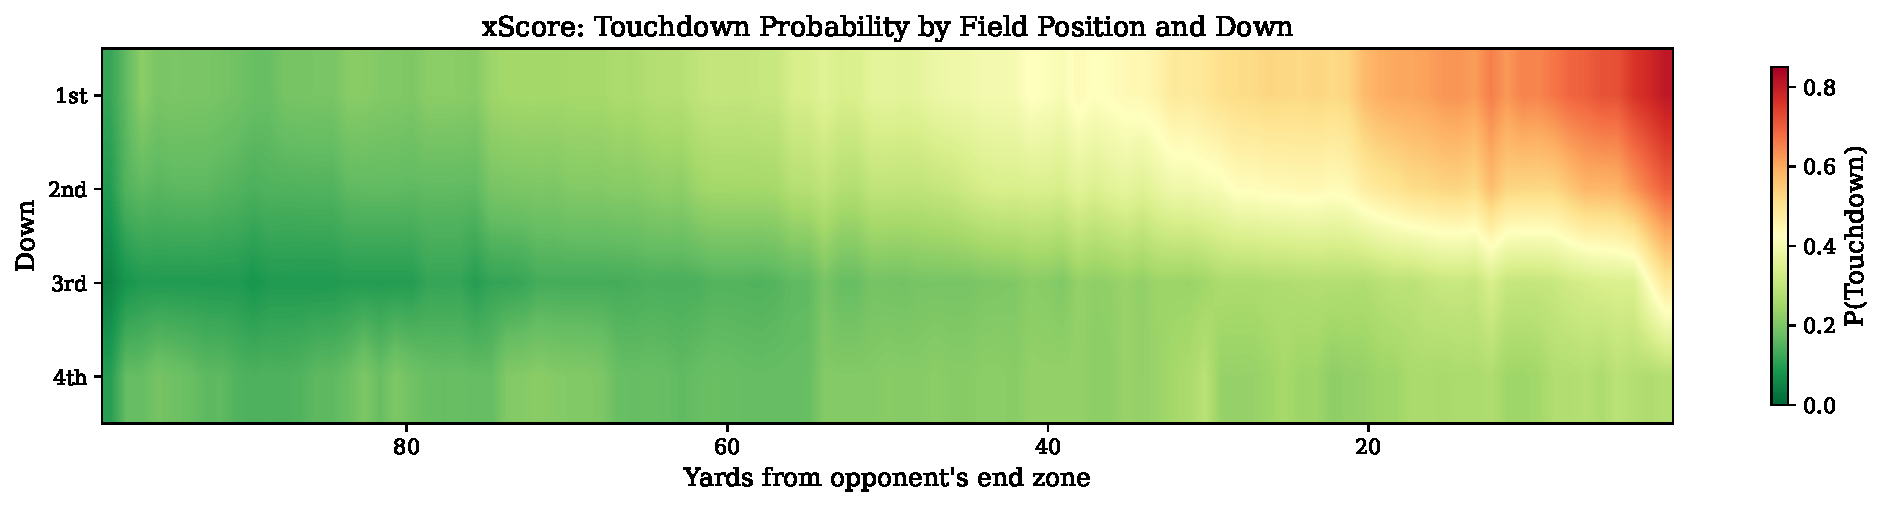
\includegraphics[width=\textwidth]{../../thesis/figures/fig2_field_heatmap.pdf}
  \caption{\xscore{} touchdown probability surface by field position and down (10 yards to go, neutral game state).}
  \label{fig:heatmap}
\end{figure}

\subsection{Summary}

Phase 1 achieves Brier 0.1562 (BSS = 15.3\% versus naive baseline, 4.1\% versus logistic regression), generalizes to pre-2018 eras (OOD Brier 0.1529), calibrates well across all four classes (mean ECE = 0.010), produces domain-consistent probability surfaces, and recovers the expected feature hierarchy. It is adopted as the primary model for downstream applications.

% ============================================================
% 6. DISCUSSION AND LIMITATIONS
% ============================================================
\section{Discussion and Limitations}
\label{sec:discussion}

\subsection{Different Targets: Why \xscore{} and EPA Are Not Competitors}

A natural question is how \xscore{} compares to EPA on the same test set. The answer is that a direct calibration comparison between the two is not appropriate because they estimate fundamentally different quantities. The \texttt{nflfastR} expected points model answers: ``what is the expected \emph{next-score differential} from this game state?'' -- a quantity that incorporates both the current drive's production and future opponent scoring expectations, spanning multiple possessions. \xscore{} answers a narrower question: ``what will \emph{this drive} produce for the possessing team?'' The two outputs have different units, different temporal scopes, and different sign conventions. Comparing their calibration curves would be comparing predictions of different targets on the same data -- a category error, not an empirical test.

This distinction clarifies the contribution: \xscore{} does not replace EPA for its intended purpose (marginal play value within a game-level framework), but provides a calibrated drive-outcome model that EPA was not designed to be. EPA's design objective is within-game leverage; \xscore{}'s is between-team quality measurement. A controlled study comparing various EPA aggregation schemes against \xscore{} drive-outcome probabilities on matched drives -- with explicit target alignment -- remains an important avenue for future work.

\subsection{The Contribution: A Measurement Instrument}

While constituent methods -- XGBoost, isotonic calibration, drive-level analysis -- are individually well-understood, their integration into a purpose-built measurement instrument for team quality evaluation has not previously appeared in the peer-reviewed literature. The specific combination -- multinomial four-class prediction at the drive level, per-class calibration producing reliable expected-point baselines, team identity deliberately excluded -- solves the particular deficiencies that arise when play-level EPA is repurposed for team quality decomposition. This instrument models what a drive \emph{will produce} given its starting state, rather than summing what each constituent play \emph{did produce} after the fact. The distinction is not merely aggregation level: it eliminates within-drive attribution problems, conditions on game state to account for play-calling effects, and preserves the distributional information that a single continuous sum discards.

\subsection{Comparison with Existing Approaches}

Table~\ref{tab:comparison} positions \xscore{} relative to existing metrics across five evaluation axes, including an honest trade-off axis where existing approaches retain advantages.

\begin{table}[htbp]
  \centering
  \caption{Comparison of NFL performance measurement approaches. Checkmarks indicate the property is satisfied.}
  \label{tab:comparison}
  \small
  \begin{tabular}{lccccc}
    \toprule
     & \rotatebox{60}{Public/verifiable} & \rotatebox{60}{Calibrated} & \rotatebox{60}{Drive-level} & \rotatebox{60}{Distributional} & \rotatebox{60}{Play-level granularity} \\
    \midrule
    EPA (nflfastR) & \checkmark &  -- &  -- &  -- & \checkmark \\
    DVOA (FO) &  -- & ? &  -- &  -- &  -- \\
    PFF &  -- &  -- &  -- &  -- & \checkmark \\
    WP (nflfastR) & \checkmark & $\sim$ &  -- &  -- & \checkmark \\
    \xscore{} & \checkmark & \checkmark & \checkmark & \checkmark &  -- \\
    \bottomrule
  \end{tabular}
\end{table}

The trade-off is explicit: \xscore{} sacrifices play-level granularity for drive-level calibration and distributional output. EPA retains play-level detail that enables within-drive attribution, individual-play evaluation, and broader community adoption. For applications requiring play-level resolution -- receiver separation analysis, blocking evaluation, individual player grades -- EPA remains the appropriate tool. For applications requiring calibrated drive-outcome expectations -- team quality decomposition, fourth-down decision modeling, expected-point baselines -- \xscore{} provides a purpose-built alternative.

\subsection{Temporal Robustness}

The OOD result confirms that field position and down are structural features of American football rather than artifacts of a specific rule regime. If the marginally superior OOD performance reflects distributional shift in 2025 (explanation 2 from Section~\ref{sec:results}), periodic retraining on updated data would maintain calibration -- a practical consideration rather than a fundamental limitation of the methodology.

\subsection{Downstream Application}

In a companion paper \citep{mecha2026gds}, \xscore{} predictions are aggregated into a Game Deserved Score framework for three-component team quality decomposition (offense, defense, special teams). This represents one application; the calibrated probability output is equally suited to fourth-down decision modeling (comparing expected points under go/punt/kick decisions given the current state), drive-quality filtering (identifying drives where teams substantially over- or under-performed expectations), and in-game strategy optimization grounded in calibrated outcome distributions.

\subsection{Limitations}

\paragraph{Data scope.}
The model conditions only on publicly observable situational features. Player tracking data (Next Gen Stats), personnel groupings, defensive coverage, and weather are absent. These omissions add noise to individual drive predictions but should not introduce systematic bias at the season level if effects are approximately symmetric across teams.

\paragraph{Temporal scope.}
The 2018--2024 training window coincides with an offense-favoring rule environment. The probability surface may be partially era-specific. Periodic recalibration on updated data would be required if future rule changes rebalance the offensive-defensive equilibrium.

\paragraph{Training distribution versus application.}
The model trains on all plays within drives but is applied to drive-start states for xEP calculation. If calibration degrades at drive-start positions specifically -- where the model has less mid-drive information about eventual outcome -- reported Brier scores may be optimistic for the xEP application. Future work should evaluate drive-start-only calibration explicitly.

\paragraph{Lookup table approximation.}
The field-position-dependent turnover penalty uses observed actual points rather than model-predicted values, avoiding circularity but introducing lookup-table approximation error for rare yardline positions with few observations. Smoothing or a secondary model could improve precision at extreme field positions.

% ============================================================
% 7. CONCLUSION
% ============================================================
\section{Conclusion}
\label{sec:conclusion}

We introduced \xscore{}, the first publicly available, calibrated, drive-level expected-points model for the NFL. The multinomial formulation predicts four drive outcomes and converts these to expected points via a field-position-dependent weighted formula that avoids circularity by relying on observed outcomes rather than recursive model predictions. The model achieves a Brier score of 0.1562 (BSS = 15.3\% versus naive baseline), generalizes across eras (OOD Brier 0.1529 on 2014--2017 data), calibrates well across all four outcome classes (mean ECE = 0.010), and learns a domain-consistent feature hierarchy confirmed by SHAP analysis.

By providing a transparent, calibrated probability baseline that is independent of team identity, \xscore{} enables downstream team quality measurement, fourth-down decision analysis, and coaching evaluation without dependence on proprietary systems. The complete codebase, trained model, and data pipeline are publicly available for replication, critique, and extension. Full methodological details, extended robustness analyses, and downstream applications are available in \citet{mecha2026xscore}.

Extensions warranting future investigation include: (1) drive-start-specific calibration evaluation, (2) a context-dependent turnover penalty replacing the lookup table with a secondary model, (3) player-level attribution decomposing team-level value to individuals, (4) quantitative comparison with drive-aggregated EPA on matched test sets with aligned targets, and (5) longer temporal windows as additional seasons become available. In a companion paper \citep{mecha2026gds}, we demonstrate \xscore{}'s application to a three-component team quality decomposition framework that enables direct comparison of offensive and defensive contributions to competitive success.

% ============================================================
% DATA AND CODE AVAILABILITY
% ============================================================
\section*{Data and Code Availability}

All play-by-play data are publicly available via the \texttt{nflfastR} package \citep{carl2021nflfastr}. The complete analytical codebase -- including model training, isotonic calibration, evaluation, and figure generation -- is available at \url{https://github.com/lasse5mecha/nfl-xscore-gds}.

% ============================================================
% CONFLICTS OF INTEREST
% ============================================================
\section*{Conflicts of Interest}

The author declares no conflicts of interest.

% ============================================================
% AI DISCLOSURE
% ============================================================
\section*{Statement on Use of Artificial Intelligence}

This paper was developed with the assistance of Claude (Anthropic), a large language model used as a coding and writing tool. All research design decisions, modeling choices, and interpretation of results are solely the author's intellectual contributions. AI-generated code was reviewed and validated by the author.

% ============================================================
% REFERENCES
% ============================================================
\printbibliography

\end{document}
